%!TEX root = ../dokumentation.tex

\section{Architektur der Anwendung}
Im folgenden Abschnitt soll die Architektur der Implementierung erläutert werden. Des Weiteren wird beleuchtet, welche Funktionen von \acs{Redis} eingesetzt werden.
\\Wie bereits im vorangegangen Abschnitt erwähnt, soll eine Chat-App implementiert werden. Die Anwendung besteht aus zwei Hauptkomponenten: dem Backend und dem Frontend (vgl. Abbildung \ref{fig:arch}). Die Aufgabe des Frontend ist es dem Benutzer eine grafische Oberfläche zu präsentieren. Alle Eingaben des Benutzers werden im Backend ausgewertet. Zwischen beiden Komponenten besteht eine bidirektionale Kommunikation. Das Frontend sendet den Input des Benutzers und das Backend sendet nötige Änderungen.
\begin{figure}[h]
	\centering
	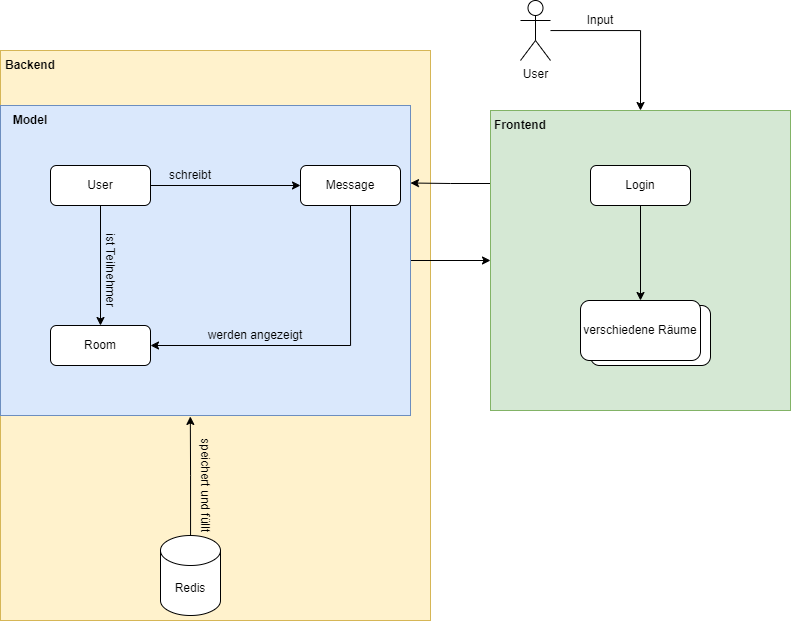
\includegraphics[width=0.8\textwidth]{redis_arch.png}
	\caption{Architektur der Chat-App}
	\label{fig:arch}
\end{figure}
\\Das Backend besteht aus zwei Teilen. Zum einen aus dem Model der Applikation, zum Anderen aus einer \acs{Redis}-Datenbank (vgl. Abbildung \ref{fig:arch}). Das Model ist ein objektorientierter Ansatz zur Modellierung der benötigten Daten. Es besteht aus einer \textit{User} Klasse, welche alle Informationen, wie Name, E-Mail und Passwort eines User speichert, einer \textit{Message} Klasse, welche Nachrichten repräsentiert, die ein User in einen bestimmten Raum sendet und einer \textit{Room} Klasse, welche einen spezifischen Chatraum darstellt. Jedes \textit{Room} Objekt hat zwei Teilnehmer und eine Menge an Nachrichten.
\\In der \acs{Redis}-Datenbank werden verschiedene Datentypen verwendet, um jeweils die Stärken dieser zu zeigen. Die verwendeten Datentypen sind Hashes und Sorted Sets (vgl. \autoref{subsec:datentypen}). Für die Speicherung der User-Daten wurden Hashes verwendet. Mit dieser Herangehensweise kann jeder User anhand eines Schlüssels identifiziert werden (vgl. Abbildung \ref{fig:sub1}). 
\\Die Räume wurden mithilfe von Sorted-Sets realisiert. Ein Raum besteht stets aus zwei Teilnehmern und einer Menge an Nachrichten. Die Teilnehmer werden mittels den festen Scores \textit{-2} und \textit{-1} identifiziert. Bei Abfrage dieser Score liefert die Datenbank den Schlüssel des zugehörigen Users. Alle weiteren Scores sind die Timestamps der zugehörigen Nachricht, welche in einem JSON ähnlichen Format abgespeichert wird (vgl. Abbildung \ref{fig:sub3}).
\\In \acs{Redis} ist es möglich Bilder in Form einer Bitmap zu speichern. Die Avatare ( = Profilbilder der User) werden ebenfalls in Sorted Sets gespeichert. Diese sind als Bitmap abgelegt und können anhand ihres Scores abgefragt und in der Applikation zurück in ein Bild umgewandelt werden (vgl. Abbildung \ref{fig:sub3}).
\begin{figure}[h]
	\centering
	
	\begin{subfigure}{0.3\textwidth}
		\centering
		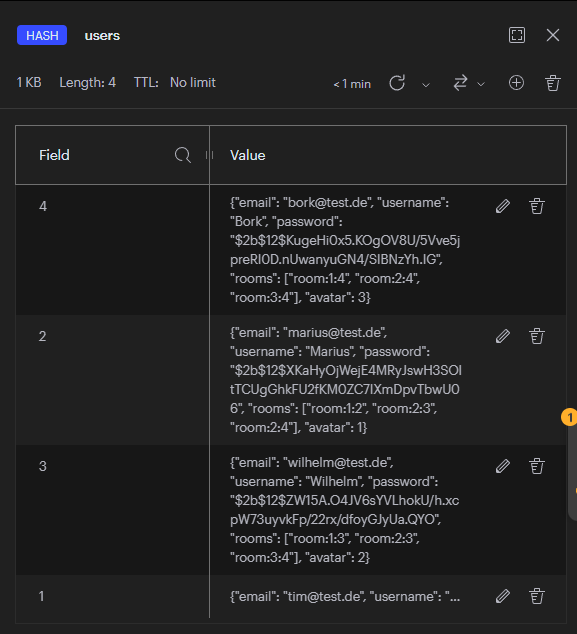
\includegraphics[width=\linewidth]{user_hash.png}
		\caption{Speicherung der User in \acs{Redis}}
		\label{fig:sub1}
	\end{subfigure}%
	\hspace{0.02\textwidth}
	\begin{subfigure}{0.3\textwidth}
		\centering
		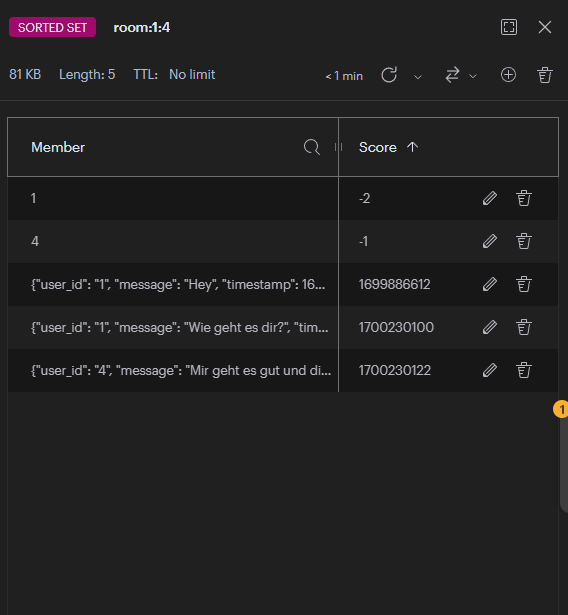
\includegraphics[width=\linewidth]{room.png}
		\caption{Speicherung der Räume in \acs{Redis}}
		\label{fig:sub2}
	\end{subfigure}%
	\hspace{0.02\textwidth}
	\begin{subfigure}{0.3\textwidth}
		\centering
		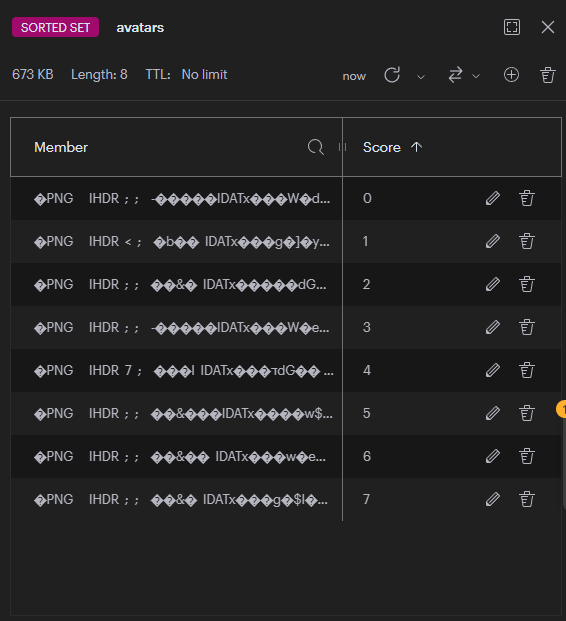
\includegraphics[width=\linewidth]{avatars.png}
		\caption{Speicherung der Avatare in \acs{Redis}}
		\label{fig:sub3}
	\end{subfigure}
	
	\caption{Datenmodellierung in \acs{Redis}}
	\label{fig:overall}
\end{figure}